\section{Dimensioning}

The dimensioning process involves optimizing the Recycling Folded-Cascode (RFC) OTA design to achieve the specified performance goals while adhering to the given constraints. Hence, a python script was created according to the analysis made in section \ref{sec:TheoreticalAnalysys}. This script showed how varying different parameters affected the circuit behavior and calculated the size of all transistors respecting size ratios. 

In order to have a more modular script three dictionaries were created to save all transistors characteristics and a list with all transistors names making the list iterable.

As a starting point all transistors sizes were set to have length of $\SI{600}{\nano\meter}$ and a $V_{DSsat} = \SI{100}{\milli\volt}$, to ensure the devices were operating in the moderate inversion region, as specified in Table \ref{tab:goals}. Then the gain equation was analyzed in order to find the transistors affected this value.

\subsection{DC gain analysis}
\label{sec:DCGain}
In order to achieve the DC gain goal of $\SI{66}{\decibel}$, it is important to first identify the devices that will influence this value and specifically what parameters. Table \ref{tab:GainTransistors}, shows the devices characteristics that affect gain, this was done by analysing \ref{eq:Av}.

\begin{table}[H]
    \centering
    \caption{Transistor's characteristics that affect gain}
    \begin{tabularx}{\textwidth}{>{\centering\arraybackslash}X >{\centering\arraybackslash}X >{\centering\arraybackslash}X}
        \toprule
        \textbf{Transistor} & \textbf{$V_{DSsat}$} & \textbf{$L_{size}$} \\
        \midrule
        $M_{3}$ & $\checkmark$ & $\checkmark$\\
        \midrule
        $M_{2a}$ & $\checkmark$ & $\times$\\
        \midrule
        $M_{1b}$ & $\checkmark$ & $\times$\\
        \midrule
        $M_{5}$ & $\checkmark$ & $\checkmark$\\
        \midrule
        $M_{11}$ & $\times$ & $\checkmark$\\
        \midrule
        $M_{7a}$ & $\times$ & $\checkmark$\\
        \bottomrule
    \end{tabularx}
    \label{tab:GainTransistors}
\end{table}

To visualize how each parameter influence the gain value independently, the gain function was plotted varying one parameter at a time, creating the graphs shown in Figure \ref{fig:GainVariation}. 

\begin{figure}[H]
    \centering
    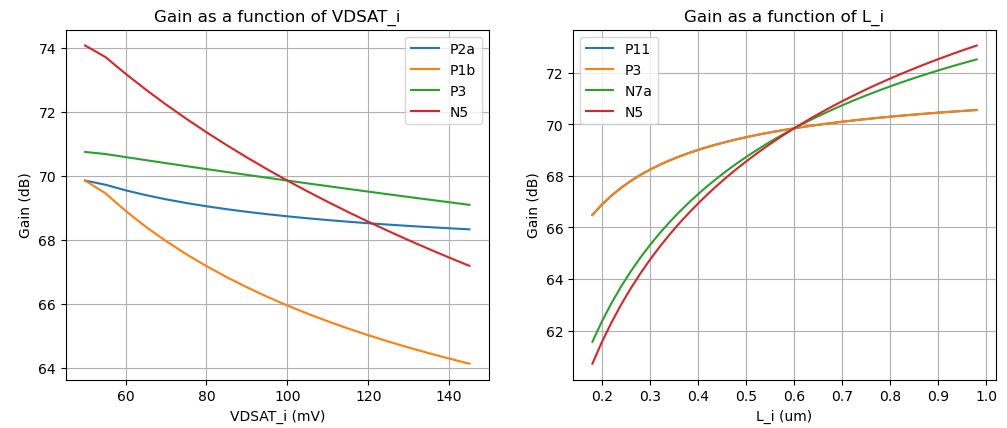
\includegraphics[width=1\textwidth]{Images/GainVariation.png}
    \caption{Gain as a function of $V_{DSsat}$ and $L_{size}$}
    \label{fig:GainVariation}
\end{figure}

As shown by Figure \ref{fig:GainVariation}, the parameters that are more relevant are, $M_{5}$ and $M_{1b}$ $V_{DSsat}$ and $M_{5}$ and $M_{7a}$ length size.

Knowing this, a heatmap was plotted, Figure \ref{fig:GainHeatMap}. The heatmap provides a more complete picture by displaying the combined influence of both variables on the gain function. Each cell in the heatmap corresponds to a specific pair of values for the two variables, with the color intensity indicating the resulting gain.

\begin{figure}[H]
    \centering
    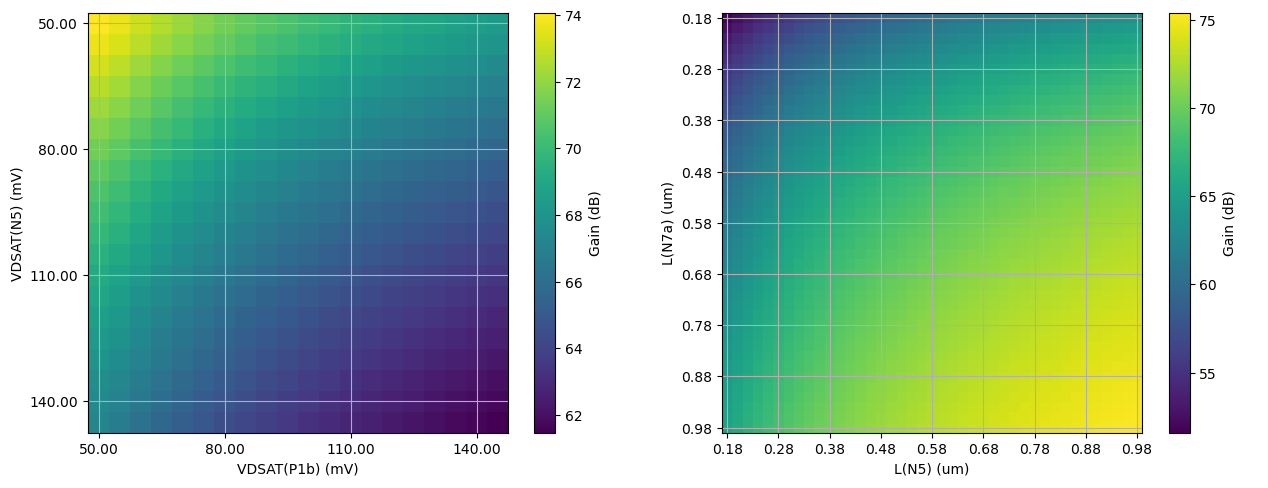
\includegraphics[width=1\textwidth]{Images/GainHeatMap.png}
    \caption{Gain HeatMap}
    \label{fig:GainHeatMap}
\end{figure}


\subsection{Gain Bandwidth Product (GBW) analysis}
\label{sec:GBWPython}
Analogously to the subsection \ref{sec:DCGain}, to achieve the Gain Bandwidth Product (GBW) target of $\SI{100}{\mega\hertz}$, the devices and parameters that influence this performance metric must be identified. Using equation \ref{eq:GBW}, the table \ref{tab:GBWTransistors} was constructed.

\begin{table}[H]
    \centering
    \caption{Transistor's characteristics that affect gain}
    \begin{tabularx}{\textwidth}{>{\centering\arraybackslash}X >{\centering\arraybackslash}X >{\centering\arraybackslash}X}
        \toprule
        \textbf{Transistor} & \textbf{$V_{DSsat}$} & \textbf{$L_{size}$} \\
        \midrule
        $M_{3}$ & $\checkmark$ & $\checkmark$\\
        \midrule
        $M_{2a}$ & $\checkmark$ & $\times$\\
        \midrule
        $M_{1b}$ & $\checkmark$ & $\times$\\
        \midrule
        $M_{5}$ & $\checkmark$ & $\checkmark$\\
        \bottomrule
    \end{tabularx}
    \label{tab:GBWTransistors}
\end{table}

Again to visualize how each parameter influence the GBW independently, the GBW function was plotted varying each parameter at a time, yielding Figure \ref{fig:GBWVariation}.

\begin{figure}[H]
    \centering
    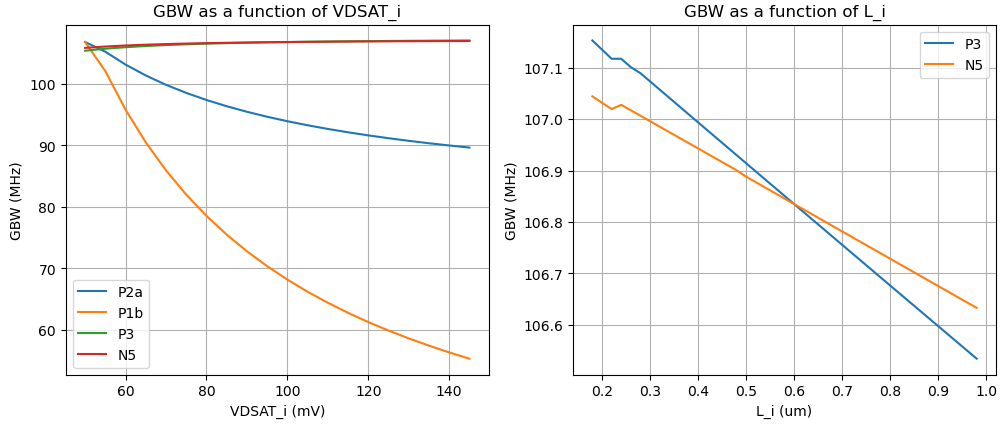
\includegraphics[width=1\textwidth]{Images/GBWVariation.png}
    \caption{GBW as a function of $V_{DSsat}$ and $L_{size}$}
    \label{fig:GBWVariation}
\end{figure}

Because for $V_{DSsat}$, devices $M_{1b}$ and $M_{2a}$ change the GBW value more drastically and for $L_{size}$ there are only two devices that affect the final value, a heatmap was plotted, yielding Figure \ref{fig:GBWHeatMap}. 

\begin{figure}[H]
    \centering
    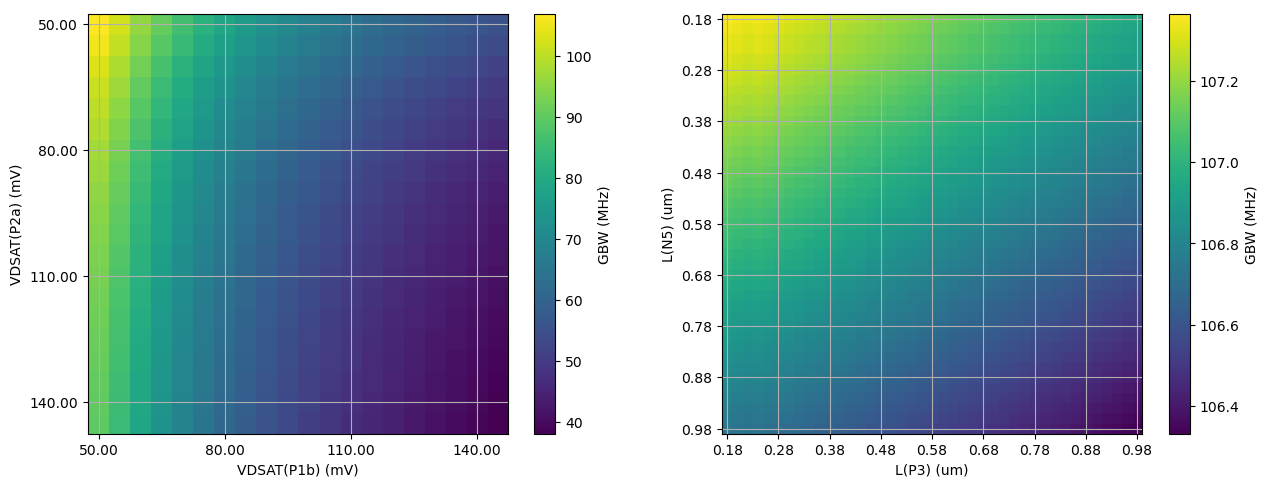
\includegraphics[width=1\textwidth]{Images/GBWHeatMap.png}
    \caption{GBW HeatMap}
    \label{fig:GBWHeatMap}
\end{figure}

\subsection{Pole Frequencies analysis}

To ensure the OTA stability, particularly in closed loop, it is important to be able to shift the poles to higher frequencies in case they do not meet specification. That is why it is important to plot how the poles behave when change transistors parameters. It is also important to note that at this stage the order in which the poles appear is not obvious, because depending on the final devices characteristics, poles can switch place.  

Because almost all poles depend on the $V_{DSsat}$ and $L_{size}$ of all devices that appear in it's equation, there was no distinction made between the devices in the $V_{DSsat}$ an $L_{size}$ plots.

\begin{figure}[H]
    \centering
    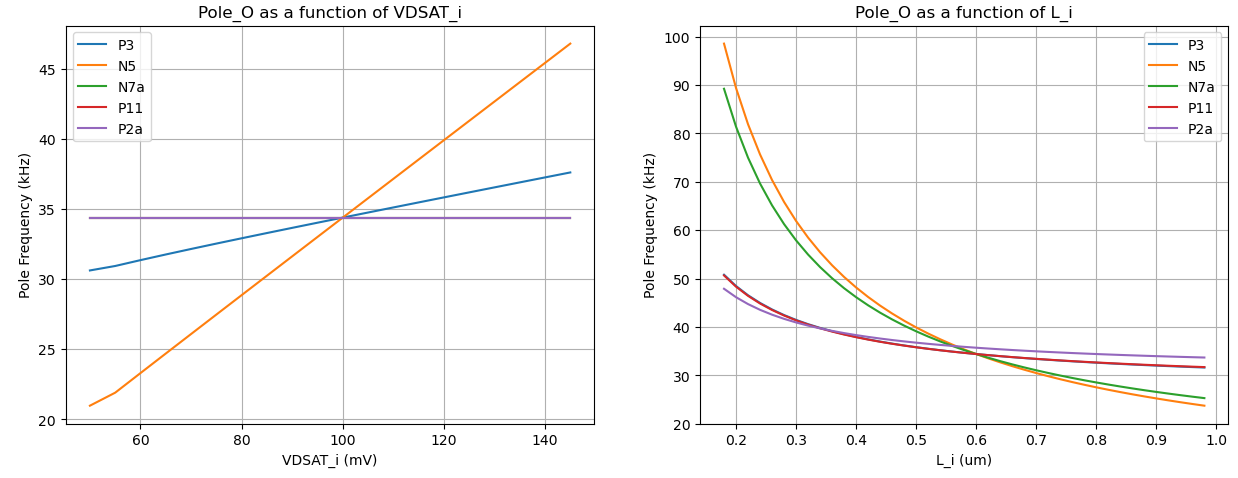
\includegraphics[width=1\textwidth]{Images/PoPlot.png}
    \caption{Output Pole as a function of $V_{DSsat}$ and $L_{size}$}
    \label{fig:PoPlot}
\end{figure}

For the first it is the least relevant, since it only affects GBW and that parameter was already explored in section \ref{sec:GBWPython}.

\begin{figure}[H]
    \centering
    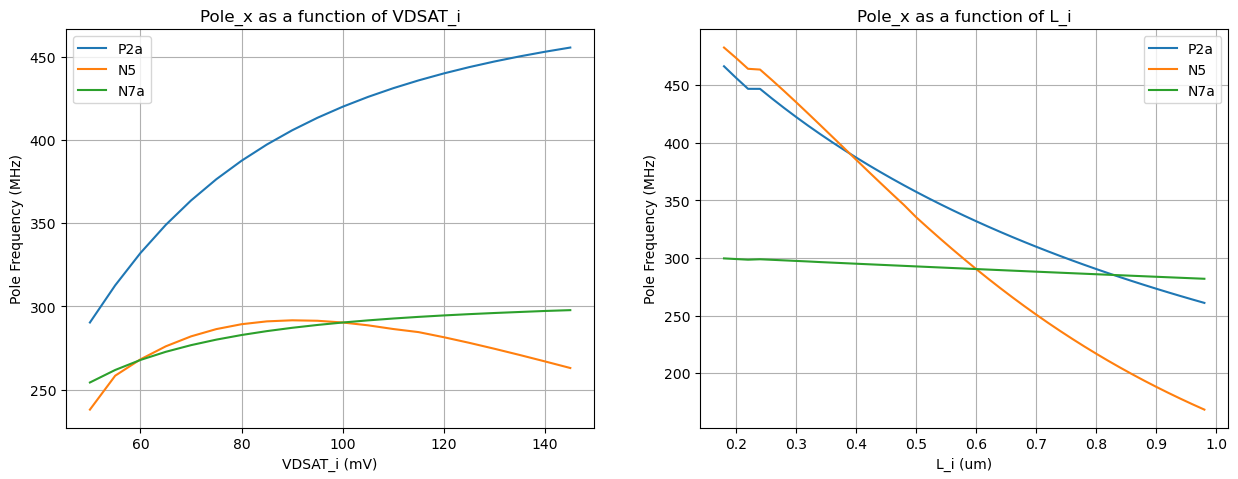
\includegraphics[width=1\textwidth]{Images/PxPlot.png}
    \caption{Pole $x$ as a function of $V_{DSsat}$ and $L_{size}$}
    \label{fig:PxPlot}
\end{figure}

As seen in Figure \ref{fig:PxPlot}, $M_{2a}$ $V_{DSsat}$ and $M_5$ $L_{size}$ are the characteristics that affect the pole $x$ frequency the most. It is also important to note that the pole frequency is not linear with the $M_5$ $V_{DSsat}$.  

\begin{figure}[H]
    \centering
    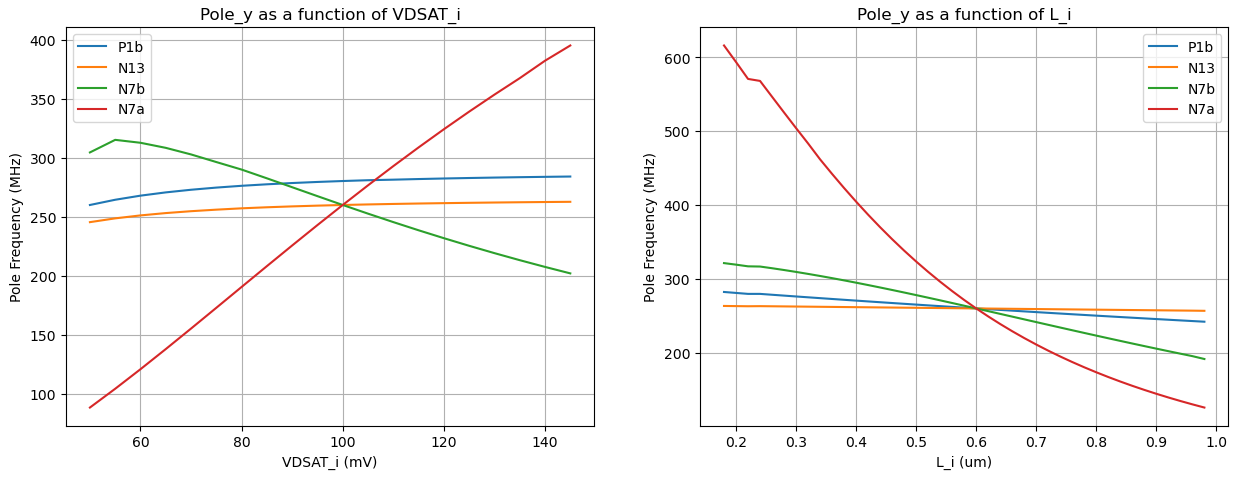
\includegraphics[width=1\textwidth]{Images/PyPlot.png}
    \caption{Pole $y$ as a function of $V_{DSsat}$ and $L_{size}$}
    \label{fig:PyPlot}
\end{figure}

For pole $y$ the most important device is $M_{7a}$, as seen in Figure \ref{fig:PyPlot}, this will be relevant later since this is also one of the most important devices for gain.

\begin{figure}[H]
    \centering
    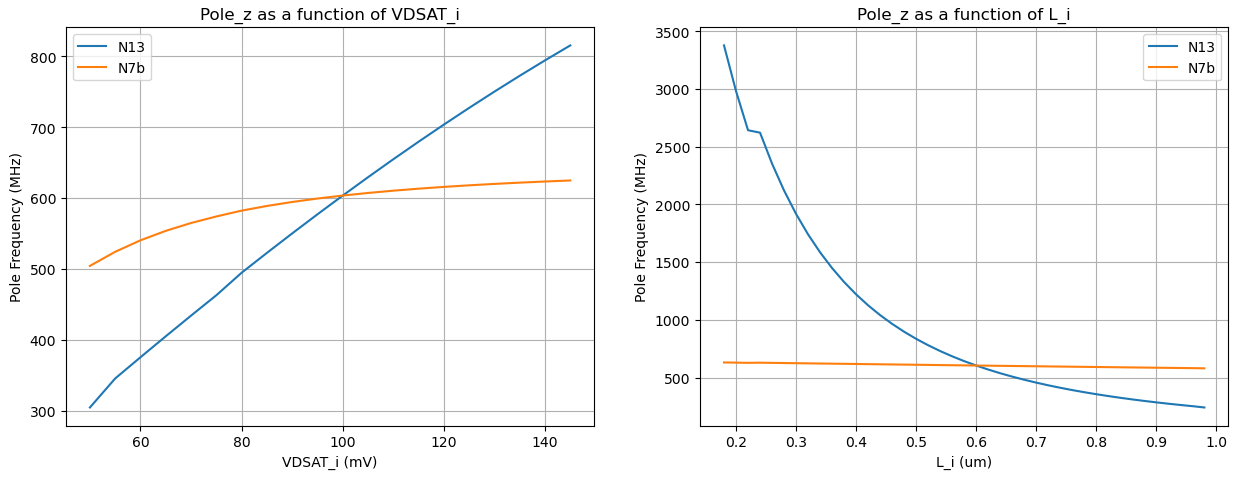
\includegraphics[width=1\textwidth]{Images/PzPlot.png}
    \caption{Pole $z$ as a function of $V_{DSsat}$ and $L_{size}$}
    \label{fig:PzPlot}
\end{figure}

Pole $z$ is generally in high frequencies as seen in Figure \ref{fig:PzPlot}, hence, this poles should not influence the OTA stability.

\begin{figure}[H]
    \centering
    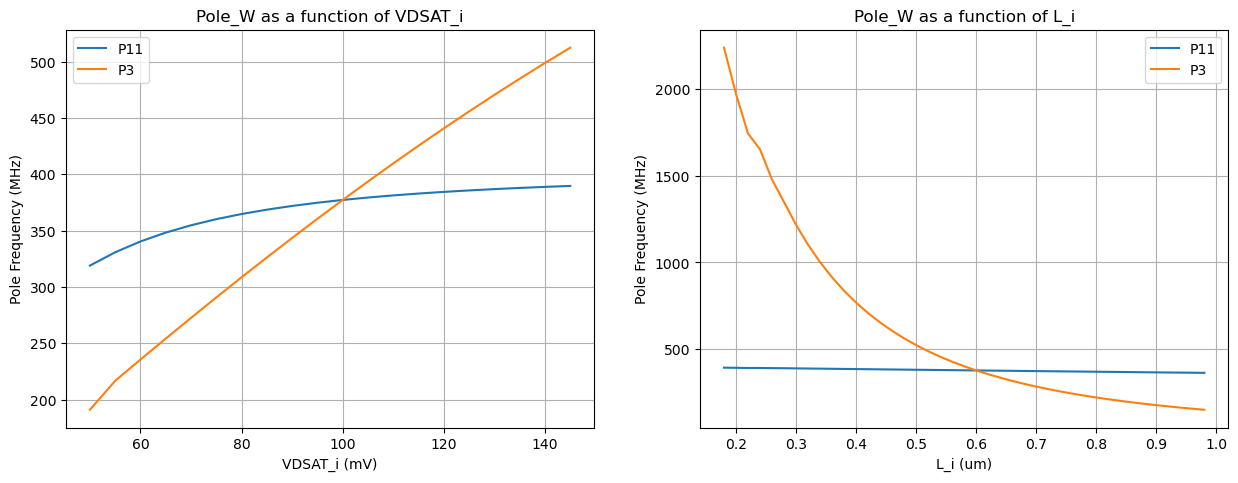
\includegraphics[width=1\textwidth]{Images/PwPlot.png}
    \caption{Pole $w$ as a function of $V_{DSsat}$ and $L_{size}$}
    \label{fig:PwPlot}
\end{figure}

Similarly to pole $z$, pole $w$, also should not be a problem for stability, but in some extreme cases it can be a problem, as depicted in Figure \ref{fig:PwPlot}, with very low $V_{DSsat}$ the pole frequency can reach the $\SI{200}{\mega\hertz}$ mark, but this region is easily avoided with a low $L_{size}$ and reasonable $V_{DSsat}$ for devices $M_{11}$ and $M_3$.

\subsection{Output Swing (OS) analysis}

\subsection{Excess-Noise Factor (ENF) analysis}

Evaluating equation \ref{eq:ENF}, we may conclude that the ENF value only depends on the $V_{DSsat}$ of devices $M_{7a}$,$M_{2a}$ and $M_{11}$. By evaluating Figure \ref{fig:enfVariation} the device that affects ENF more predominantly is $M_{2a}$, this device $V_{DSsat}$ must be relatively small.

\begin{figure}[H]
    \centering
    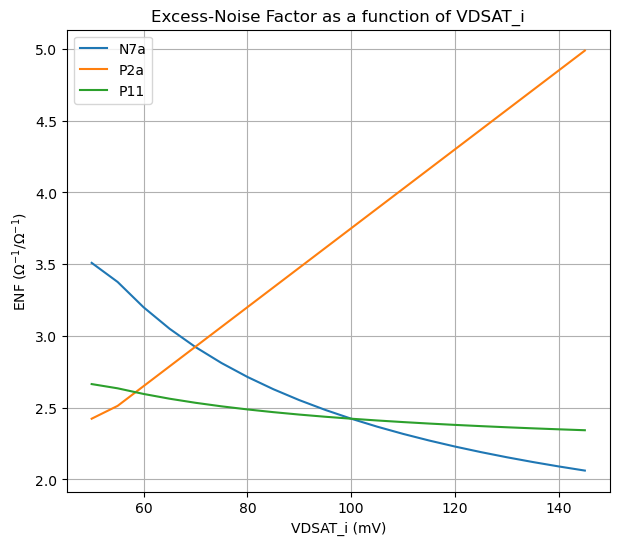
\includegraphics[width=0.5\textwidth]{Images/enfVariation.png}
    \caption{Excess-Noise Factor as function of $V_{DSsat}$}
    \label{fig:enfVariation}
\end{figure}

\subsection{Power Consumption analysis}

\subsection{Merit Figure and Results}

\subsection{Dimensioning Strategy}

dizer que fizemos um algoritmo no python para chegar aos valores otimos dos transistores.

\subsection{Final Transistors Sizing}

Before dimensioning all devices is important to identify which transistors are independent, meaning, which transistors sizes do not depend on the size of other transistors. This list of transistors will be the free variables and are shown in table \ref{tab:FreeMos}.


\begin{table}[h]
    \centering
    \caption{Independent transistors.}
    \begin{tabularx}{\textwidth}{>{\centering\arraybackslash}X 
                                >{\centering\arraybackslash}X 
                                >{\centering\arraybackslash}X  
                                >{\centering\arraybackslash}X
                                >{\centering\arraybackslash}X
                                >{\centering\arraybackslash}X
                                >{\centering\arraybackslash}X
                                >{\centering\arraybackslash}X
        }
        \toprule
        $M_{1b}$ & $M_{2a}$ & $M_{3}$ & $M_{11}$ & $M_{5}$ & $M_{7a}$ & $M_{9}$ & $M_{b3}$ \\
        \bottomrule
    \end{tabularx}
    \label{tab:FreeMos}
\end{table}

As way to identify if the circuit meets the goals and constraints set in table \ref{tab:goals}, this values must be printed and are colour coded to identify if they meet specification. Then, all transistors sizes are printed with the finger number calculated to make introducing this values in cadence easier. 

With the knowledge of how the circuit behaves, the devices dimensions must be finally selected. In order to have with a decent starting point, a simple optimization function was developed. This function works by iterating all devices from table \ref{tab:FreeMos}, and finding which combination of $V_{DSsat}$ and $L_{size}$ gave the best value for a second $FoM$ value, this different Figure of Merit is needed to take into account the output swing, gain and ENF, since the current value is not change in this function it is not taken into account for this second $FoM$. The final equation is equation \ref{eq:FoM2}. It is important to note that the function that calculates this value, returns a negative number if any of the specification is not met.

\begin{equation}
    \label{eq:FoM2}
    FoM_2 = \frac{GBW\cdot OS \cdot Gain}{ENF}
\end{equation}

The final dimensions of the transistors were calculated using the python script and are shown in Table \ref{tab:WL-teo}.

\begin{table}[H]
    \centering
    \caption{Transistors theoretical final dimensions}
    \begin{tabularx}{\textwidth}{>{\centering\arraybackslash}X >{\centering\arraybackslash}X >{\centering\arraybackslash} X >{\centering\arraybackslash}X}
        \toprule
        \textbf{Transistor} & \textbf{Width (W)} & \textbf{Length (L)} & \textbf{Fingers}\\
        \midrule
        $M_{B1}, \ M_{B2}, \ M_{B4}$ & \SI{2.84}{\micro\meter} & \SI{180}{\nano\meter} &  1\\
        \midrule
        $M_{B3}, \ M_{B7}$ & \SI{1.69}{\micro\meter} & \SI{180}{\nano\meter} & 1\\
        \midrule
        $M_{B5}$ & \SI{6.48}{\micro\meter} & \SI{800}{\nano\meter} & 1\\
        \midrule
        $M_{B6}$ & \SI{34.08}{\micro\meter} & \SI{600}{\nano\meter} & 1\\
        \midrule
        $M_{1a}, \ M_{2a}, \ M_{1b}, \ M_{2b}$ & \SI{9.465}{\micro\meter} & \SI{400}{\nano\meter} & 6\\
        \midrule
        $M_{3}, \ M_{4}$ & \SI{7.7425}{\micro\meter} & \SI{200}{\nano\meter} & 8\\
        \midrule
        $M_{5}, \ M_{6}$ & \SI{8.15}{\micro\meter} & \SI{800}{\nano\meter} & 4\\
        \midrule
        $M_{7a}, \ M_{8a}$ & \SI{8.505}{\micro\meter} & \SI{500}{\nano\meter} & 10\\
        \midrule
        $M_{7b}, \ M_{8b}$ & \SI{5.89}{\micro\meter} & \SI{180}{\nano\meter} & 2\\
        \midrule
        $M_{9}$ & \SI{6.9675}{\micro\meter} & \SI{180}{\nano\meter} & 4\\
        \midrule
        $M_{10}, \ M_{11}$ & \SI{8.519}{\micro\meter} & \SI{600}{\nano\meter} & 10\\
        \midrule
        $M_{12}, \ M_{13}$ & \SI{4.24}{\micro\meter} & \SI{180}{\nano\meter} & 1\\
        \bottomrule
    \end{tabularx}
    \label{tab:WL-teo}
\end{table}

The final values for each transistor $V_{DSsat}$ and $I_D$ current can be found in table \ref{tab:TeoVDSsatId}.

\begin{table}[H]
    \centering
    \caption{Theoretical values for $V_{DSsat}$ and $I_D$}
    \begin{tabularx}{\textwidth}{>{\centering\arraybackslash}X >{\centering\arraybackslash}X >{\centering\arraybackslash}X}
        \toprule
        \textbf{Transistor} & \textbf{$V_{DSat}$} & \textbf{$I_D$}\\
        \midrule
        $M_{1a}$ & \SI{-50}{\milli\volt} & \SI{-25}{\micro\ampere}\\
        \midrule
        $M_{1b}$ & \SI{-50}{\milli\volt} & \SI{-25}{\micro\ampere}\\
        \midrule
        $M_{2a}$ & \SI{-50}{\milli\volt} & \SI{-25}{\micro\ampere}\\
        \midrule
        $M_{2b}$ & \SI{-50}{\milli\volt} & \SI{-25}{\micro\ampere}\\
        \midrule
        $M_{3}$ & \SI{-50}{\milli\volt} & \SI{-50}{\micro\ampere}\\
        \midrule
        $M_{4}$ & \SI{-50}{\milli\volt} & \SI{-50}{\micro\ampere}\\
        \midrule
        $M_{5}$ & \SI{100}{\milli\volt} & \SI{50}{\micro\ampere}\\
        \midrule
        $M_{6}$ & \SI{100}{\milli\volt} & \SI{50}{\micro\ampere}\\
        \midrule
        $M_{7a}$ & \SI{60}{\milli\volt} & \SI{75}{\micro\ampere}\\
        \midrule
        $M_{7b}$ & \SI{60}{\milli\volt} & \SI{25}{\micro\ampere}\\
        \midrule
        $M_{8a}$ & \SI{60}{\milli\volt} & \SI{75}{\micro\ampere}\\
        \midrule
        $M_{8b}$ & \SI{60}{\milli\volt} & \SI{25}{\micro\ampere}\\
        \midrule
        $M_{9}$ & \SI{100}{\milli\volt} & \SI{-100}{\micro\ampere}\\
        \midrule
        $M_{10}$ & \SI{-50}{\milli\volt} & \SI{-25}{\micro\ampere}\\
        \midrule
        $M_{11}$ & \SI{-50}{\milli\volt} & \SI{-25}{\micro\ampere}\\
        \midrule
        $M_{12}$ & \SI{100}{\milli\volt} & \SI{25}{\micro\ampere}\\
        \midrule
        $M_{13}$ & \SI{100}{\milli\volt} & \SI{25}{\micro\ampere}\\
        \bottomrule
    \end{tabularx}
    \label{tab:TeoVDSsatId}
\end{table}


\begin{table}[H]
    \centering
    \caption{Theoretical values for $V_{DSsat}$ and $I_D$ with fixed current}
    \begin{tabularx}{\textwidth}{>{\centering\arraybackslash}X >{\centering\arraybackslash}X >{\centering\arraybackslash}X}
        \toprule
        \textbf{Transistor} & \textbf{$V_{DSat}$} & \textbf{$I_D$}\\
        \midrule
        $M_{1a}$ & \SI{-50}{\milli\volt} & \SI{-25}{\micro\ampere}\\
        \midrule
        $M_{1b}$ & \SI{-50}{\milli\volt} & \SI{-25}{\micro\ampere}\\
        \midrule
        $M_{2a}$ & \SI{-50}{\milli\volt} & \SI{-25}{\micro\ampere}\\
        \midrule
        $M_{2b}$ & \SI{-50}{\milli\volt} & \SI{-25}{\micro\ampere}\\
        \midrule
        $M_{3}$ & \SI{-50}{\milli\volt} & \SI{-50}{\micro\ampere}\\
        \midrule
        $M_{4}$ & \SI{-50}{\milli\volt} & \SI{-50}{\micro\ampere}\\
        \midrule
        $M_{5}$ & \SI{100}{\milli\volt} & \SI{50}{\micro\ampere}\\
        \midrule
        $M_{6}$ & \SI{100}{\milli\volt} & \SI{50}{\micro\ampere}\\
        \midrule
        $M_{7a}$ & \SI{60}{\milli\volt} & \SI{75}{\micro\ampere}\\
        \midrule
        $M_{7b}$ & \SI{60}{\milli\volt} & \SI{25}{\micro\ampere}\\
        \midrule
        $M_{8a}$ & \SI{60}{\milli\volt} & \SI{75}{\micro\ampere}\\
        \midrule
        $M_{8b}$ & \SI{60}{\milli\volt} & \SI{25}{\micro\ampere}\\
        \midrule
        $M_{9}$ & \SI{100}{\milli\volt} & \SI{-100}{\micro\ampere}\\
        \midrule
        $M_{10}$ & \SI{-50}{\milli\volt} & \SI{-50}{\micro\ampere}\\
        \midrule
        $M_{11}$ & \SI{-50}{\milli\volt} & \SI{-50}{\micro\ampere}\\
        \midrule
        $M_{12}$ & \SI{100}{\milli\volt} & \SI{25}{\micro\ampere}\\
        \midrule
        $M_{13}$ & \SI{100}{\milli\volt} & \SI{25}{\micro\ampere}\\
        \bottomrule
    \end{tabularx}
    \label{tab:TeoVDSsatIdFix}
\end{table}


\begin{table}[H]
    \centering
    \caption{Transistors with fixed current}
    \begin{tabularx}{\textwidth}{>{\centering\arraybackslash}X >{\centering\arraybackslash}X >{\centering\arraybackslash} X >{\centering\arraybackslash}X}
        \toprule
        \textbf{Transistor} & \textbf{Width (W)} & \textbf{Length (L)} & \textbf{Fingers}\\
        \midrule
        $M_{B1}, \ M_{B2}, \ M_{B4}$ & \SI{2.84}{\micro\meter} & \SI{180}{\nano\meter} &  1\\
        \midrule
        $M_{B3}, \ M_{B7}$ & \SI{1.69}{\micro\meter} & \SI{180}{\nano\meter} & 1\\
        \midrule
        $M_{B5}$ & \SI{6.48}{\micro\meter} & \SI{800}{\nano\meter} & 1\\
        \midrule
        $M_{B6}$ & \SI{8.52}{\micro\meter} & \SI{600}{\nano\meter} & 4\\
        \midrule
        $M_{1a}, \ M_{2a}, \ M_{1b}, \ M_{2b}$ & \SI{9.47}{\micro\meter} & \SI{400}{\nano\meter} & 6\\
        \midrule
        $M_{3}, \ M_{4}$ & \SI{7.7425}{\micro\meter} & \SI{200}{\nano\meter} & 8\\
        \midrule
        $M_{5}, \ M_{6}$ & \SI{8.17}{\micro\meter} & \SI{800}{\nano\meter} & 4\\
        \midrule
        $M_{7a}, \ M_{8a}$ & \SI{8.505}{\micro\meter} & \SI{500}{\nano\meter} & 10\\
        \midrule
        $M_{7b}, \ M_{8b}$ & \SI{5.89}{\micro\meter} & \SI{180}{\nano\meter} & 2\\
        \midrule
        $M_{9}$ & \SI{6.9675}{\micro\meter} & \SI{180}{\nano\meter} & 4\\
        \midrule
        $M_{10}, \ M_{11}$ & \textcolor{red}{\SI{9.47}{\micro\meter} } & \SI{600}{\nano\meter} & 18\\
        \midrule
        $M_{12}, \ M_{13}$ & \SI{4.24}{\micro\meter} & \SI{180}{\nano\meter} & 1\\
        \bottomrule
    \end{tabularx}
    \label{tab:WL-teo-fix}
\end{table}